%%%%%
% CH4 %
%%%%%

\chapter{Transient heat conduction}
	Let's Imagine that we want to cool a bottle of beer. What time will it take ? We will consider 3 different cases neglecting sometimes convection sometimes conduction. 
	
\section{Lumped systems analysis}
	\begin{wrapfigure}[6]{l}{3cm}
	\vspace{-5mm}
	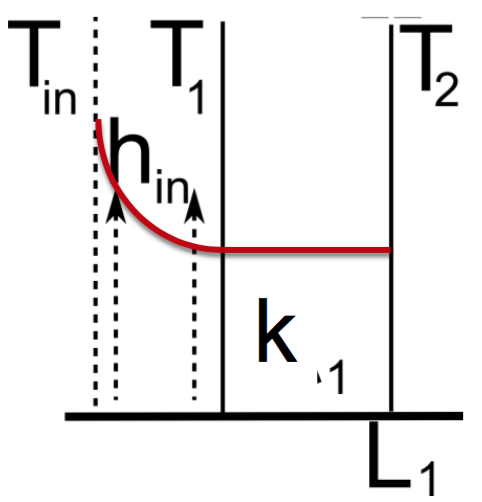
\includegraphics[scale=0.3]{ch3/8}
	\end{wrapfigure}	
	Let's study the case where convection is the limitative factor for heat (dispersion of heat within the solid is negligible compared to heat arrival to the surface). Let's remind the expression of the Biot number (go to \autoref{sec:3.3.3})
	\begin{equation}
		Bi = \frac{L_1h_{in}}{k_1}
	\end{equation}
	
	\subsection{Calculation of lumped systems}
		Let's consider an object of volume $V$ and surface $A$ initially to temperature $T_i$ that we put into an infinite temperature $T_\infty$ enviroment. We want to know what happens. So my accumulation, is equal to the amount that comes with the convection
		\begin{equation}
			V\rho c_p \frac{\partial T}{\partial t} = A h(T_\infty - T)
		\end{equation}
		Integrating and applying the initial condition $t = 0 \rightarrow T = T_i$
		\begin{equation}
			\underbrace{\frac{T-T_\infty}{T_i - T_\infty}}_{\theta} =
			 \exp \left( - \frac{Ah}{V\rho c_p}t \right) = 
			 \exp \left( - \underbrace{\frac{Vh}{Ak}}_{Bi} \underbrace{\frac{A^2k}{V^2\rho c_p}t}_{Fo} \right) 
		\end{equation}
It can always be expressed like a function of theta. 
The expression in the $\exp$ must be undimentional so we will make it appear. $V/A$ = lenght, so the definition of Biot number appears. The other is including t and is called the \textbf{Fourrier number}. 
	
	
	
	